\def\linkdethi{} %Đường link cần dẫn tới
\anmaQR
%%%%%%%%%%%%%%%%%%%%%%%%
\def\toanlop{12}
\def\thoigian{90}
\def\namhoc{2025 - 2026}
\begin{dethi}
	{Bộ GD\&ĐT}
	{VTED ft KING EDU}
	{TDMT01}
	{Đề thi thử THPTQG 2026}
\end{dethi}
\caulc
\Opensolutionfile{ans}[ans/ansTN-Dung]
%%%=============EX_1=============%%%
\begin{ex}%[2D1N1-1]%[TDMT01]%[Nguyễn Trí Minh Tuấn]
	Hàm số $y=x^3-3x^2+1$ nghịch biến trên khoảng
	\choice
	{\True $(0;2)$}
	{$(-\infty;0)$}
	{$(2;+\infty)$}
	{$(0;+\infty)$}
	\loigiai{
		Ta có $y=x^3-3x^2+1$.\\
		Suy ra $y'=3x^2-6x$.\\ 
		Khi đó $y'=0 \Leftrightarrow \hoac{&x=0\\&x=2.}$\\
		Bảng xét dấu
		\begin{center}
			
\begin{tikzpicture}
				\tkzTabInit[nocadre=false,lgt=1.2,espcl=3]
				{$x$/0.7,$y'$/0.7}
				{$-\infty$,$0$,$2$,$+\infty$}
				\tkzTabLine{,+,0,-,0,+,}
			\end{tikzpicture}
		\end{center}
		Vậy hàm số $y=x^3-3x^2+1$ nghịch biến trên khoảng $(0;2)$.
	}
\end{ex}
%%%=============================%%%

%%%=============EX_2=============%%%
\begin{ex}%[1D6N3-3]%[TDMT01]%[Trần Văn Thiện]
	Tập giá trị của hàm số $y=\mathrm{e}^x$ là
	\choice
	{$\mathbb{R}\setminus \{0 \}$}
	{$\mathbb{R}$}
	{\True $\left(0; +\infty\right)$}
	{$\left(\mathrm{e}; +\infty\right)$}
	\loigiai{
		Hàm số $y=\mathrm{e}^x$ là hàm số mũ có cơ số $\mathrm{e}>1$ nên luôn đồng biến trên $\mathbb{R}$.\\
		Ngoài ra ta có $\lim\limits_{x\to -\infty} y = 0$ và $\lim\limits_{x\to +\infty} y = +\infty$.\\ 
		Do đó tập giá trị của hàm số là $(0; +\infty)$.
	}
\end{ex}
%%%=============================%%%

%%%=============EX_3=============%%%
\begin{ex}%[1D3N1-2]%[TDMT01]%[Phạm Hải Dương]
	Giá trị của $\lim\limits_{n\to +\infty} \dfrac{2n+3}{n+1}$ bằng
	\choice
	{$3$}
	{\True $2$}
	{$+\infty$}
	{$1$}
	\loigiai{
		Ta có $\lim\limits_{n\to +\infty}\dfrac{2n+3}{n+1}=\lim\limits_{n\to +\infty}\dfrac{n\left(2+\dfrac{3}{n}\right)}{n\left(1+\dfrac{1}{n}\right)}= \lim\limits_{n\to +\infty}\dfrac{2+\dfrac{3}{n}}{1+\dfrac{1}{n}}=2$.
	}
\end{ex}
%%%=============================%%%

%%%=============EX_4=============%%%
\begin{ex}%[1H8H4-2]%[TDMT01]%[Văn Minh Thoại]
	\immini[thm]{Cho hình chóp $S.ABC$ có cạnh bên $SA\perp(ABC)$. Phát biểu nào dưới đây \textbf{sai}?
		\choice
		{$SA\perp AB$}
		{$(SAB)\perp (ABC)$}
		{$SA\perp BC$}
		{\True $(SBC)\perp (ABC)$}
	}{ 	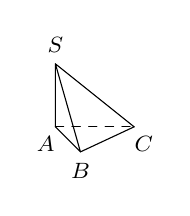
\begin{tikzpicture}[declare function={goc=-45; a=5; b=0.45*a; h=4;},line join=round,line cap=round,>=stealth,scale=0.2]
			\path
			(0,0) coordinate (A)--+(0,h) coordinate (S)
			(a,0) coordinate (C)
			(goc:b) coordinate (B);
			\draw[dashed] (A)--(C);
			\draw (S)--(B)
			(S)--(A)--(B)--(C)--cycle;
			\foreach \x/\goc in {S/90,A/240,C/-60,B/-90}
			\fill (\x) node[shift={(\goc:7pt)},font = \footnotesize]{$\x$} circle (1pt);
		\end{tikzpicture}
	}
	\loigiai{
		Vì $SA\perp (ABC)$ nên $SA\perp AB$ và $SA\perp BC$ là phát biểu đúng.\\
		Ngoài ra, vì $\heva{&SA \perp (ABC) \\ & SA \subset (SAB)}$ nên $(SAB) \perp (ABC)$ cũng là phát biểu đúng.
	}
\end{ex}
%%%=============================%%%

%%%=============EX_5=============%%%
\begin{ex}%[2D1N1-2]%[TDMT01]%[Lê Phúc]
	Cho hàm số $f(x)$ có bảng biến thiên như hình vẽ bên dưới. Hỏi hàm số $f(x)$ \textbf{đồng biến} trên khoảng nào dưới đây?
	\begin{center}
		\begin{tikzpicture}[font=\normalsize,t style/.style={style=solid}]
			\tkzTabInit[nocadre=false, lgt=1.2, espcl=2.5, deltacl=0.5]
			{$x$/0.75, $f(x)$/3}
			{$-\infty$, $-3$, $0$, $2$, $+\infty$}
			\path
			($(N12)!0.1!(N11)$) node (A1){$ -\infty $}
			($(N22)!0.8!(N21)$) node (A2){$ 4 $}
			($(N32)!0.25!(N31)$) node (A3){$ -2 $}
			($(N42)!0.65!(N41)$) node (A4){$ 3 $}
			($(N52)!0.1!(N51)$) node (A5){$ -\infty $};
			\foreach \x/\y in {A1/A2, A2/A3, A3/A4, A4/A5}{
				\draw[-stealth] (\x)--(\y);
			}
		\end{tikzpicture}
	\end{center}
	\choice
	{$(-\infty;-1)$}
	{\True $(0;2)$}
	{$(2;+\infty)$}
	{$(-3;0)$}
	\loigiai{
		Dựa vào bảng biến thiên ta thấy hàm số $f(x)$ đồng biến trên khoảng $(0;2)$.
	}
\end{ex}
%%%=============================%%%

%%%=============EX_6=============%%%
\begin{ex}%[1D2N3-4]%[TDMT01]%[Vũ Hồng Toàn]
	Cho cấp số nhân $(u_n)$ có số hạng đầu bằng $2$ và công bội bằng $3$. Hãy tính $u_3$.
	\choice
	{\True $18$}
	{$54$}
	{$8$}
	{$27$}
	\loigiai{
		Áp dụng công thức tổng quát của cấp số nhân $u_n=u_1\cdot q^{n-1}$ ta có $u_3 = u_1 \cdot q^2 = 2 \cdot 3^2 = 18$.
	}
\end{ex}
%%%=============================%%%

%%%=============EX_7=============%%%
\begin{ex}%[1D6H4-3]%[TDMT01]%[Chu Ha]
	Tập nghiệm của bất phương trình $\log(x-1)<\log(5-2x)$ là
	\choice
	{$(-\infty;2)$}
	{$\{1;2\}$}
	{$\left(1;\dfrac{5}{2}\right)$}
	{\True $(1;2)$}
	\loigiai{
		Điều kiện xác định $\heva{&x - 1 > 0\\& 5 -2x >0}\Leftrightarrow 1 < x < \dfrac{5}{2}$.\\
		Khi đó ta có 
		\allowdisplaybreaks
		\begin{align*}
			&\ \log(x-1)<\log(5-2x) \\
			\Leftrightarrow&\ x-1<5-2x \\
			\Leftrightarrow&\ x<2.
		\end{align*}
		Kết hợp với điều kiện xác định $1 < x < \dfrac{5}{2}$, ta được tập nghiệm của bất phương trình đã cho là $S=(1;2)$.
	}
\end{ex}
%%%=============================%%%

%%%=============EX_8=============%%%
\begin{ex}%[1D5H1-3]%[TDMT01]%[Nguyễn Sơn Thành]
	Cho hai mẫu số liệu ghép nhóm $M_1$, $M_2$ với bảng tần số ghép nhóm như sau
	\begin{center}
		Nhóm $M_1$
		\begin{tabular}{|c|c|c|c|c|c|c|}
			\hline
			Nhóm & $\left[2;3\right)$ &$\left[3;4\right)$ &$\left[4;5\right)$ &$\left[5;6\right)$ &$\left[6;7\right)$ &$\left[7;8\right)$ \\
			\hline
			Tần số $M_1$ & $4$ & $3$ & $6$ & $4$ & $5$ & $4$ \\
			\hline
		\end{tabular}
	\end{center}
	
	\begin{center}
		Nhóm $M_2$
		\begin{tabular}{|c|c|c|c|c|c|c|}
			\hline
			Nhóm &$\left[6;9\right)$ &$\left[9;12\right)$ &$\left[12;15\right)$ &$\left[15;18\right)$ &$\left[18;21\right)$ &$\left[21;24\right)$ \\
			\hline
			Tần số $M_2$ & $8$ & $6$ & $12$ & $8$ & $10$ & $8$ \\
			\hline
		\end{tabular}
	\end{center}
	Gọi $\overline{x}_1$, $\overline{x}_2$ lần lượt là số trung bình cộng của hai mẫu số liệu $M_1$, $M_2$. Hãy chọn mệnh đề \textbf{đúng}.
	\choice
	{\True $\overline{x}_2=3\overline{x}_1$}
	{$\overline{x}_2=6\overline{x}_1$}
	{$\overline{x}_2=2\overline{x}_1$}
	{$\overline{x}_2=\overline{x}_1$}
	\loigiai{ Ta có
		\begin{itemize}
			\item $\overline{x}_1=\dfrac{2{,}5 \cdot 4+3{,}5\cdot3 + 4{,}5\cdot6+ 5{,}5\cdot4+6{,}5\cdot5+7{,}5\cdot4}{4+3+6+4+5+4}=\dfrac{132}{26}=\dfrac{66}{13}$.
			\item $\overline{x}_2=\dfrac{7{,}5 \cdot 8+10{,}5\cdot6 + 13{,}5\cdot12+ 16{,}5\cdot8+19{,}5\cdot10+22{,}5\cdot8}{8+6+12+8+10+8}=\dfrac{792}{52}=\dfrac{198}{13}$.
		\end{itemize}
		Vậy $\overline{x}_2=3\overline{x}_1$.
	}
\end{ex}
%%%=============================%%%

%%%=============EX_9=============%%%
\begin{ex}%[1H8N7-4]%[TDMT01]%[Đỗ Đường Hiếu]
	Cho hình lăng trụ đứng $ABCD.A'B'C'D'$ có đáy $ABCD$ là hình vuông cạnh bằng $2$ và cạnh bên $AA'=3$. Tính thể tích của hình lăng trụ $ABC.A'B'C'$.
	\choice
	{$V=12$}
	{$V=4$}
	{\True $V=6$}
	{$V=2$}
	\loigiai{
		\immini{
			Ta có $V_{ABC.A'B'C'}=S_{ABC}\cdot AA'=\dfrac{1}{2}\cdot 2^2\cdot 3 = 6$.\\
			Vậy thể tích của hình lăng trụ $ABC.A'B'C'$ bằng $6$.}
		{\begin{tikzpicture}[scale=1, font=\footnotesize, line join=round, line cap=round, >=stealth, declare function={a=2; b=0.45*a; h=0.65*a;}]
				\path (0:0) coordinate (A)
				(220:b) coordinate (B)
				($(B)+(a,0)$) coordinate (C)
				(a,0) coordinate (D)
				\foreach \x in {A,B,C,D}{(\x)++(90:h) coordinate (\x1)};
				\draw[dashed] (A1)--(A)--(B) (A)--(D);
				\draw (B1)--(A1)--(D1)--(C1) (D1)--(D)--(C) (B)--(C)--(C1)--(B1)--cycle;
				\foreach \x/\goc/\t in {A/45/A,B/-90/B,C/-90/C,D/0/D,A1/90/A',B1/90/B',C1/90/C',D1/90/D'}
				\fill (\x) circle (1pt) node[shift={(\goc:7pt)},font=\scriptsize]{$\t$};
		\end{tikzpicture}}
	}
\end{ex}
%%%=============================%%%

%%%=============EX_10=============%%%
\begin{ex}%[2D1N1-1]%[TDMT01]%[Huỳnh Quốc Đạt]
	Hàm số $y=\dfrac{x+2}{x-1}$
	\choice
	{nghịch biến trên tập xác định}
	{đồng biến trên từng khoảng xác định}
	{đồng biến biến trên tập xác định}
	{\True nghịch biến trên từng khoảng xác định}
	\loigiai{
		Tập xác định $\mathscr{D}=\mathbb{R}\setminus\{1\}$.\\
		Ta có $y=\dfrac{x+2}{x-1}$.\\
		Suy ra $y'=\dfrac{-3}{(x-1)^2}<0$, $\forall x \neq 1$.\\
		Do đó hàm số nghịch biến trên từng khoảng xác định $(-\infty;1)$ và $(1;+\infty)$.
	}
\end{ex}
%%%=============================%%%

%%%=============EX_11=============%%%
\begin{ex}%[1D9N1-3]%[TDMT01]%[Dương Công Tạo]
	Cho hai biến cố độc lập $A$, $B$ của một phép thử $T$. Mệnh đề  \textbf{đúng} là
	\choice
	{\True $\mathrm{P}(AB)=\mathrm{P}(A)\cdot \mathrm{P}(B)$}
	{$\mathrm{P}(AB)=0$}
	{$\mathrm{P}(A\cup B)=\mathrm{P}(A)+\mathrm{P}(B)$}
	{$\mathrm{P}(AB)=\mathrm{P}(A)+\mathrm{P}(B)$}
	\loigiai{
		Vì $A$, $B$ là hai biến cố độc lập nên ta có $\mathrm{P}(A\cap B)=\mathrm{P}(A)\cdot \mathrm{P}(B)$.
	}
\end{ex}
%%%=============================%%%

%%%=============EX_12=============%%%
\begin{ex}%[1D1H4-6]%[TDMT01]%[Nguyễn Tấn Linh]
	Giá trị lớn nhất của hàm số $y=2\sin x + 3\cos x$ là
	\choice
	{$5$}
	{$13$}
	{\True $\sqrt{13}$}
	{$3$}
	\loigiai
	{
		Ta có
		\begin{eqnarray*}
			y&=&2\sin x + 3\cos x\\
			&=&\sqrt{13}\left(\dfrac{2}{\sqrt{13}}\sin x+ \dfrac{3}{\sqrt{13}}\cos x\right)\\
			&=&\sqrt{13}\sin(x+\alpha),
		\end{eqnarray*}
		trong đó $\alpha$ là góc thỏa $\heva{&\sin \alpha = \dfrac{3}{\sqrt{13}}\\ &\cos\alpha=\dfrac{2}{\sqrt{13}}}.$\\
		Vì $\sin(x+\alpha)\leq 1$ nên $\sqrt{13}\sin(x+\alpha)\leq 1$.\\
		Vậy giá trị lớn nhất của hàm số là $\sqrt{13}$.
	}
\end{ex}
%%%=============================%%%
\Closesolutionfile{ans}

\cauds
\Opensolutionfile{ans}[ans/ansTN-DungSai]
%%%=============EX_13=============%%%
\begin{ex}%[2D1V3-4]%[TDMT01]%[Duong Xuan Loi]
	Cho hàm số $f(x)=7^x-1-6x$.
	\choiceTF[t]
	{\True $f'(x)=7^x\ln 7-6$}
	{\True $f'(x)=0\Leftrightarrow x= \log_7 \dfrac{6}{\ln 7}$}
	{\True $f(x)=0 \Rightarrow x \in \{0;1;3\}$}
	{Có tất cả $4$ giá trị nguyên của $x$ thỏa mãn $7^{x^2-2x}+12x-6x^2 \leq 1$}
	\loigiai{
		\begin{itemchoice}
			\itemch Ta có $f'(x)=7^x\ln 7 -6$.
			\itemch Ta có $f'(x)=0\Leftrightarrow 7^x=\dfrac{6}{\ln 7}\Leftrightarrow x= \log_7 \dfrac{6}{\ln 7}$.
			\itemch Hàm số $f(x)$ có đạo hàm $f'(x) = 7^x \ln 7 - 6$.\\
			Ta thấy đạo hàm đổi dấu đúng một lần tại $x_0 = \log_7 \dfrac{6}{\ln 7} \approx 0{,}58$.\\ 
			Do đó hàm số có tối đa $2$ nghiệm.\\
			Ta nhẩm được $x=0$ và $x=1$ là hai nghiệm của $f(x)=0$.\\ Tập nghiệm của phương trình là $S = \{0; 1\}$.\\
			Vì $S \subset \{0; 1; 3\}$ nên mệnh đề \lq\lq $f(x) = 0 \Rightarrow x \in \{0; 1; 3\}$\rq\rq\ là mệnh đề đúng.
			\itemch Đặt $u=x^2-2x$, bất phương trình trở thành $7^u-6u-1 \leq 0 \Leftrightarrow f(u) \leq 0$.\\
			Bảng xét dấu của $f(x)$
			\begin{center}
				
\begin{tikzpicture}
					\tkzTabInit[nocadre=false,deltacl=0.5,espcl=3,lgt=1.2]
					{$x$/0.7,$f(x)$/0.7}
					{$-\infty$,$0$,$1$,$+\infty$}
					\tkzTabLine{,+,0,-,0,+,}
				\end{tikzpicture}
			\end{center}
			Từ bảng xét dấu $f(x)$ ta có $f(x) \leq 0 \Leftrightarrow 0 \leq x \leq 1$.\\
			Vậy $f(u) \leq 0 \Leftrightarrow 0 \leq u \leq 1 \Leftrightarrow 0 \leq x^2-2x \leq 1$.\\
			Giải hệ bất phương trình
			\[ \heva{&x^2-2x \geq 0 \\&x^2-2x \leq 1} \Leftrightarrow \heva{&\hoac{& x \leq 0 \\& x \geq 2} \\&1-\sqrt{2} \leq x \leq 1+\sqrt{2}} \Leftrightarrow \hoac{& 1-\sqrt{2} \leq x \leq 0 \\& 2 \leq x \leq 1+ \sqrt{2}.} \]
			Vì $x \in \mathbb{Z}$ nên $x \in \{0; 2\}$.\\
			Do đó chỉ có $2$ giá trị nguyên của $x$ thỏa mãn yêu cầu bài toán. 
		\end{itemchoice}
	}
\end{ex}
%%%=============================%%%

%%%=============EX_14=============%%%
\begin{ex}%[1H8V7-8]%[TDMT01]%[Hmh]
	Cho hình chóp cụt đều $ABCD.A'B'C'D'$ có các cạnh đáy $AB=4$, $A'B'=8$, có khoảng cách $\mathrm{d}\big(A,(A'B'C'D')\big)=6$.
	\choiceTF[t]
	{\True Thể tích của hình chóp cụt đều $ABCD.A'B'C'D'$ bằng $224$}
	{\True $\mathrm{d}\big(A',(BCD)\big)=6$ (\textit{làm tròn kết quả đến hàng đơn vị})}
	{$\mathrm{d}\big(AB,C'D'\big)=10$ (\textit{làm tròn kết quả đến hàng đơn vị})}
	{$\mathrm{d}\big(AB,CC'\big)=6$ (\textit{làm tròn kết quả đến hàng đơn vị})}
	\loigiai{Gọi $I$, $J$, $E$, $H$, $L$, $O$ lần lượt là trung điểm của $AB$, $C'D'$, $CD$, $A'C'$, $A'B'$, $IE$. Khi đó ta có
		\begin{center}
			\begin{tikzpicture}[scale=0.8,font=\footnotesize,
				line join=round,line cap=round,>=stealth,every node/.style={scale=0.8}]
				\def\ab{2.5}
				\def\ac{5}
				\def\h{6}
				\path
				(0,0) coordinate (A')
				++(-140:\ab) coordinate (B')
				++(0:\ac) coordinate (C')
				($(A')+(C')-(B')$) coordinate (D')
				($(A')!1/2!(C')$) coordinate (H)
				($(H)+(0,\h)$) coordinate (S);
				\def\t{0.5} 
				\path
				($(S)!\t!(A')$) coordinate (A)
				($(S)!\t!(B')$) coordinate (B)
				($(S)!\t!(C')$) coordinate (C)
				($(S)!\t!(D')$) coordinate (D)
				($(S)!\t!(H)$) coordinate (O)
				($(A)!\t!(B)$) coordinate (I)
				($(C')!\t!(D')$) coordinate (J)
				($(C)!\t!(D)$) coordinate (E)
				($(A')!\t!(B')$) coordinate (L)
				($(S)!.7!(E)$) coordinate (K)
				($(J)!(I)!(L)$) coordinate (R);
				\foreach \i in{B',C',D'}{\draw (S)--(\i);};
				\draw (B')--(C')--(D');
				\draw[dashed] (S)--(A')--(B')
				(C')--(A')--(D')--(B')
				(S)--(H);
				\draw [dashed] (K)--(I)
				(O)--(E)
				(B)--(A)--(D)
				(J)--(I)
				(S)--(I)
				(I)--(L)--(R);
				\draw (B)--(C)--(D)
				(S)--(J);
				\draw[dashed] (I)--(R) node[midway,font=\scriptsize,right]{$6$};
				\draw[dashed] (I)--(O) node[midway,font=\scriptsize,below]{$2$};
				\draw[dashed] (I)--(O) node[midway,font=\scriptsize,below]{$2$};
				\draw[dashed] (R)--(H) node[midway,font=\scriptsize,above left]{$2$};
				\draw[dashed] (H)--(J) node[midway,font=\scriptsize,below]{$4$};
				\pic[draw,angle eccentricity=1.8,angle radius=2mm]{right angle=I--K--J};
				\path (S)--(B')--([turn]-90:15pt) coordinate (xt)
				($(S)-(B')+(xt)$) coordinate (yt);
				\draw[>=stealth,|<->|] (xt)--(yt) node[fill=white,inner sep=0pt,font=\scriptsize,pos=0.5,sloped]{4};
				\foreach \x/\y/\z in {I/L/A',I/R/H,O/H/L,E/J/D',L/J/C'}{
					\path (\y) pic[draw,angle radius=5pt]{right angle = \x--\y--\z};
				}
				\foreach \i/\g in {A'/180,B'/-180,C'/-90,D'/0,H/-90,S/90,A/40,B/-180,C/-30,D/90,I/90,J/0,E/0,O/45,K/45,L/180,R/-140}
				\fill[black] (\i) circle (1pt)+(\g:2.5mm) node[scale=1]{$\i$};
			\end{tikzpicture}
		\end{center}
		\begin{itemchoice}
			\itemch Khối chóp cụt đều $ABCD. A'B'C'D'$ có thể tích
			\[ V=\dfrac{1}{3} \cdot\left(S_1+S_2+\sqrt{S_1 S_2}\right) \cdot h	=\dfrac{1}{3} \cdot\left(4^2+8^2+\sqrt{4^2 \cdot 8^2}\right) \cdot 6 = 224.\]
			\itemch $\mathrm{d}\big(A', (BCD)\big)=\mathrm{d}\big(A' ,(ABCD)\big)=\mathrm{d}\big(A, (A'B'C'D')\big)=6$.
			\itemch
			\immini{$AB \parallel C'D' \Rightarrow \mathrm{d}\big(AB , C'D'\big)=IJ=\sqrt{6^2+6^2}=6 \sqrt{2}$ (do $IJ\perp C'D'$).}{
				\begin{tikzpicture}[scale=1, font=\footnotesize, line join=round, line cap=round, >=stealth, declare function={a=2; h=3; goc=-110;}]
					\path
					(0,0) coordinate (I)
					(a,0) coordinate (E)
					(goc:h) coordinate (L)
					($(E)+({-180-goc}:h)$) coordinate (J)
					($(L)!(I)!(J)$) coordinate (R)
					($(I)!0.5!(E)$) coordinate (O)
					($(J)!(O)!(L)$) coordinate (H);
					\foreach \x/\y in {I/L,E/J}{
						\path (\x)--(\y) node[midway,sloped]{\tikz{\draw (-90:1pt)--(90:1pt);}};
					}
					\draw (I)--(E)--(J)--(L)--cycle (I)--(R)
					(O)--(H);
					\draw (E)--(J) node[midway,font=\scriptsize,right]{$2$};
					\draw (I)--(R) node[midway,font=\scriptsize,right]{$6$};
					\path (I)--(E)--([turn]90:5pt) coordinate (xt)
					($(I)-(E)+(xt)$) coordinate (yt);
					\draw[>=stealth,|<->|] (xt)--(yt) node[fill=white,inner sep=0pt,font=\scriptsize,pos=0.5,sloped]{4};
					\path (R)--(H)--([turn]-90:4pt) coordinate (xt)
					($(R)-(H)+(xt)$) coordinate (yt);
					\draw[>=stealth,|<->|] (xt)--(yt) node[fill=white,inner sep=0pt,font=\scriptsize,pos=0.5,sloped]{2};
					\path (J)--(H)--([turn]90:4pt) coordinate (xt)
					($(J)-(H)+(xt)$) coordinate (yt);
					\draw[>=stealth,|<->|] (xt)--(yt) node[fill=white,inner sep=0pt,font=\scriptsize,pos=0.5,sloped]{4};
					\foreach \x/\y/\z in {I/R/H,O/H/J}{
						\path (\y) pic[draw,angle radius=4pt]{right angle = \x--\y--\z};
					}
					\foreach \t/\g in {I/180,E/0,J/0,L/180,R/140,O/-40,H/140}{
						\fill (\t) circle (1pt) node[shift={(\g:9pt)},font=\scriptsize]{$ \t $};
					}
			\end{tikzpicture}}
			\itemch Gọi $K$ là hình chiếu của $I$ lên $SE$.\\
			Ta có $\mathrm{d}\big(AB, CC'\big)=\mathrm{d}\big(AB,(CC'D'D)\big)=\mathrm{d}\big(AB,(SCD)\big)
			=\mathrm{d}\big(I,(SCD)\big)=\mathrm{d}\big(I, SE\big)$.\\
			Ta có $\dfrac{S O}{S H}=\dfrac{O E}{H J}=\dfrac{4}{8}=\dfrac{1}{2}	\Leftrightarrow \dfrac{S O}{S O+6}=\dfrac{1}{2} \Leftrightarrow S O=6$.\\
			Từ đó $IK=4 \cdot \sin \widehat{K E I}=4 \cdot \dfrac{6}{\sqrt{6^2+2^2}} \approx 3{,}79$.
		\end{itemchoice}
	}
\end{ex}
%%%=============================%%%

%%%=============EX_15=============%%%
\begin{ex}%[1D7V2-5]%[TDMT01]%[Lê Hồ Quang Minh]
	Cho hàm số $y=f(x)=x^3-3x+2$ có đồ thị $(C)$ và điểm $A(3;0)$.
	\choiceTF[t]
	{\True Phương trình tiếp tuyến với $(C)$ tại điểm $(2;4)$ là $y=9x-14$}
	{\True Tiếp tuyến có hệ số góc nhỏ nhất của $(C)$ là $y=-3x+2$}
	{Số đường tiếp tuyến song song với trục $Ox$ là $2$}
	{Cosin của góc tạo bởi hai đường tiếp tuyến kẻ từ $A$ đến $(C)$ bằng $0{,}65$ (\textit{làm tròn kết quả đến hàng phần trăm})}
	\loigiai{
		\begin{itemchoice}
			\itemch Ta có $f'(x)=3x^2-3$, $f'(2)=9$.\\
			Phương trình tiếp tuyến là $y=9(x-2)+4=9x-14$.
			\itemch Với $M(x_M;y_M)$ là tiếp điểm.\\ Hệ số góc tiếp tuyến của $(C)$ là $f'(x_M)=3x_M^2-3 \geq -3$.\\
			Ta có $\min f'(x_M)=-3 \Leftrightarrow x_M=0 \Rightarrow y_M=2$.\\
			Phương trình tiếp tuyến của $(C)$ tại điểm $M(0;2)$ là $y=-3(x-0)+2=-3x+2$.
			\itemch Gọi $x_0$ là hoành độ tiếp điểm.\\ Vì tiếp tuyến song song với trục hoành nên $f'(x_0)=0 \Leftrightarrow \hoac{&x_0=1\\&x_0=-1.}$
			\begin{itemize}
				\item Với $x_0=1\Rightarrow y_0=0$. Phương trình tiếp tuyến là $y=0$ (loại do trùng với trục $Ox$).
				\item Với $x_0=-1 \Rightarrow y_0=4$. Phương trình tiếp tuyến là $y=4$.
			\end{itemize}
			Vậy có $1$ tiếp tuyến song song với trục hoành.
			\itemch Gọi phương trình tiếp tuyến của $(C)$ qua $A(3;0)$ là $(d)\colon y=a(x-3)+0\Rightarrow (d)\colon y=ax-3a$.\\
			Gọi $N(x_N;y_N)$ là tiếp điểm của $d$ và $(C)$.\\
			Điều kiện tiếp xúc $\heva{&f'(x_N)=a  &&(1)\\&f(x_N)=ax_N-3a &&(2).}$\\
			Thay $(1)$ vào $(2)$ ta được 
			\allowdisplaybreaks
			\begin{eqnarray*}
				&&f(x_N)=(x_N-3)f'(x_N)\\
				&\Leftrightarrow& {x_N}^3-3x_N+2 = (x_N-3)(3{x_N}^2-3)\\
				&\Leftrightarrow& {x_N}^3-3x_N+2 = 3{x_N}^3-9{x_N}^2-3x_N+9 \\
				&\Leftrightarrow& 2{x_N}^3-9{x_N}^2+7 = 0 \\
				&\Leftrightarrow& (x_N-1)(2{x_N}^2-7x_N-7) = 0\\
				&\Leftrightarrow& \hoac{&x_N=1\\&x_N= \dfrac{7 \pm \sqrt{105}}{4}.}
			\end{eqnarray*}
			Gọi $d_1$, $d_2$, $d_3$ là $3$ tiếp tuyến kẻ từ $A$ đến $(C)$ lần lượt có hệ số góc là $k_1=f'(1)=0$, $k_2=f'\left(\dfrac{7+ \sqrt{105}}{4}\right)$, $k_3=f'\left(\dfrac{7-\sqrt{105}}{4}\right)$ từ đó ta có
			\begin{itemize}
				\item $\cos (d_1,d_2)=\dfrac{|1+k_1 k_2|}{\sqrt{1+k_1^2} \cdot \sqrt{1+k_2^2}} \approx 0{,}02$.
				\item $\cos (d_1,d_3)=\dfrac{|1+k_1 k_3|}{\sqrt{1+k_1^2} \cdot \sqrt{1+k_3^2}}\approx 0{,}7$.
				\item $\cos (d_2,d_3)=\dfrac{|1+k_2 k_3|}{\sqrt{1+k_2^2} \cdot \sqrt{1+k_3^2}}\approx 0{,}7$.
			\end{itemize}
		\end{itemchoice}
	}
\end{ex}
%%%=============================%%%

%%%=============EX_16=============%%%
\begin{ex}%[2D6V2-4]%[TDMT01]%[Lương Pho]
	Một học sinh tiến hành khoanh ngẫu nhiên $3$ câu đúng sai một cách độc lập. Mỗi câu có $4$ ý $a$, $b$, $c$, $d$. Mỗi ý chỉ có hai lựa chọn là đúng hoặc sai. Đúng $1$ ý được $0{,}1$ điểm, đúng hai ý được $0{,}25$ điểm, đúng $3$ ý được $0{,}5$ điểm, đúng $4$ ý được $1$ điểm. Tất nhiên không đúng ý nào trong một câu thì không được điểm nào.
	\choiceTF[t]
	{\True Xác suất để trong một câu khoanh được đúng một ý là $0{,}25$}
	{\True Xác suất để trong một câu đúng được ít nhất một ý là $0{,}9375$}
	{Xác suất để học sinh này được đúng $1$ điểm là $0{,}1875$}
	{Xác suất để học sinh này được đúng $2$ điểm là $0{,}0725$}
	\loigiai{
		Khoanh đúng $1$ ý xác suất là $0{,}5$; sai $1$ ý xác suất là $0{,}5$.
		\begin{itemchoice}
			\itemch Xác suất trong một câu khoanh được đúng $1$ ý, $3$ ý còn lại sai là
			\[\mathrm{C}_4^1 \cdot 0{,}5 \cdot(0{,}5)^3=0{,}25.\]
			\itemch Xác suất trong $1$ câu đúng được ít nhất $1$ ý là $1-(0{,}5)^4=0{,}9375$.
			\itemch Ta có
			\begin{itemize}
				\item Xác suất một câu được $1$ điểm là $ 0{,} 5^4=\dfrac{1}{16}$.
				\item Xác suất một câu được $0$ điểm là $ 0{,} 5^4=\dfrac{1}{16}$.
				\item Xác suất một câu được $0{,}5$ điểm là $\mathrm{C}_4^3\cdot(0{,}5)^3 \cdot 0{,}5=0{,}25=\dfrac{4}{16}$.
				\item Xác suất một câu được $0{,}25$ điểm là $\mathrm{C}_4^2\cdot(0{,}5)^2 \cdot (0{,}5)^2=\dfrac{6}{16}$.
			\end{itemize}
			\begin{enumerate}[\it TH$_1$.]
				\item Một câu được $1$ điểm và hai câu được $0$ điểm
				\[3\cdot\dfrac{1}{16}\cdot \left(\dfrac{1}{16}\right)^2=\dfrac{3}{4\,096}.\]
				\item Hai câu được $0{,}5$ điểm và một câu $0$ điểm
				\[3\cdot (0{,}25)^2\cdot\dfrac{1}{16}=\dfrac{3}{256}=\dfrac{48}{4\,096}.\]
				\item Một câu được $0{,}5$ điểm và hai câu được $0{,}25$ điểm
				\[3\cdot 0{,}25 \cdot \left(\dfrac{6}{16}\right)^2=\dfrac{27}{256}=\dfrac{432}{4\,096}.\]
			\end{enumerate}
			Xác suất để học sinh này được đúng $1$ điểm là
			\[\dfrac{3}{4\,096}+\dfrac{48}{4\,096}+\dfrac{432}{4\,096}=\dfrac{483}{4\,096}\approx 0{,}1179.\]
			\itemch
			\begin{enumerate}[\it TH$_1$.]
				\item Hai câu được $1$ điểm và một câu được $0$ điểm
				\[3\cdot \left(\dfrac{1}{16}\right)^2\cdot\dfrac{1}{16}=\dfrac{3}{4\,096}.\]
				\item Một câu được $1$ điểm và hai câu $0{,}5$ điểm
				\[3\cdot\dfrac{1}{16}\cdot (0{,}25)^2=\dfrac{3}{256}=\dfrac{48}{4\,096}.\]
			\end{enumerate}
			Xác suất để học sinh này được đúng $2$ điểm là
			\[\dfrac{3}{4\,096}+\dfrac{48}{4\,096}=\dfrac{51}{4\,096}\approx0{,}01245.\]
		\end{itemchoice}
	}
\end{ex}
%%%=============================%%%
\Closesolutionfile{ans}

\caukq
\Opensolutionfile{ans}[ans/ansTN-DienKhuyet]
%%%=============EX_17=============%%%
\begin{ex}%[1H8V5-4]%[TDMT01]%[Võ Hiệp]
	Cho hình chóp đều $S. ABCD$ có độ dài các cạnh $SA=6$, $AB=4$. Tính khoảng cách giữa hai đường thẳng $SA$ và $BD$ (\textit{làm tròn kết quả đến hàng phần mười}).
	\par
	\shortans[0]{2,5}
	\loigiai{
		\immini{
			Gọi $O$ là giao điểm của $AC$ và $BD$.\\
			Do $S. ABCD$ là hình chóp đều, nên ta có $ABCD$ là hình vuông và $SO\perp (ABCD)$.\\
			Gọi $H$ là hình chiếu của $O$ trên $SA$.\\
			Ta có
			\[\heva{&AC\perp BD &(ABCD\, \text{là hình vuông})\\& SO\perp BD &(SO\perp (ABCD))}\]
			$\Rightarrow BD\perp (SAO)\Rightarrow BD\perp OH$.\\
			Suy ra $\mathrm{d}\big(SA,BD\big)=OH$.\\
			Lại có $ABCD$ là hình vuông, $AB=4 \Rightarrow AC=4\sqrt{2}\Rightarrow AO=2\sqrt{2}$.\\
			Tam giác $SAO$ vuông tại $O$, $OH\perp SA$.\\
			Suy ra $SO^2=SA^2-AO^2=6^2-\left(2\sqrt{2}\right)^2=28$.\\
			Do đó $\dfrac{1}{OH^2}=\dfrac{1}{SO^2}+\dfrac{1}{OA^2}=\dfrac{1}{28}+\dfrac{1}{8}=\dfrac{9}{56}\Rightarrow OH=\sqrt{\dfrac{56}{9}}=\dfrac{2\sqrt{14}}{3}$.\\
			Vậy $\mathrm{d}\big(SA,BD\big)=OH=\dfrac{2\sqrt{14}}{3}\approx 2{,}5$.
		}
		{	\begin{tikzpicture}[scale=1,font=\footnotesize,line join=round,line cap=round,>=stealth]
				\tikzset{declare function={a=3; b=2; h=3.5;}}
				\path (0,0) coordinate (B)
				(a,0) coordinate (C)
				(-145:b) coordinate (A)
				($(A)+(C)$) coordinate (D)
				($(B)!0.5!(D)$) coordinate (O)
				($(O)+(0,h)$) coordinate (S)
				($(S)!(O)!(A)$) coordinate (H);
				\foreach \x/\y/\z in {B/O/S,C/O/S}{
					\path (\y) pic[draw,angle radius=5pt]{right angle = \x--\y--\z};
				}
				\draw[dashed] (A)--(B)--(C)--cycle (D)--(B)--(S)--(O)--(H);
				\draw (S)--(A)--(D)--(C)--cycle (S)--(D);
				\foreach \t/\g in {B/120,A/180,D/0,C/0,S/90,O/-90,H/180}{
					\fill (\t) circle (1pt) node[shift={(\g:7pt)},font=\scriptsize]{$\t$};
				}
			\end{tikzpicture}
		}	
	}
\end{ex}
%%%=============================%%%

%%%=============EX_18=============%%%
\begin{ex}%[2D1H1-2]%[TDMT01]%[Nguyễn Đức Tuấn Anh]
	Cho hàm số $f\left(x\right)$ có bảng biến thiên như hình vẽ bên dưới.
	\begin{center}
		\begin{tikzpicture}[font=\normalsize,t style/.style={style=solid}]
			\tkzTabInit[nocadre=false,lgt=1.2,espcl=2.5,deltacl=0.5]%,help]
			{$x$/0.75,$f'(x)$/0.75,$f (x)$/3}
			{$-\infty$,$-5$,$0$,$+\infty$}
			\tkzTabLine{,+,0,-,0,+}
			\path
			($(N13)!0.1!(N12)$) node (A1){$ -\infty $}
			($(N23)!0.65!(N22)$) node (A2){$ 4 $}
			($(N33)!0.25!(N32)$) node (A3){$ -3 $}
			($(N43)!0.8!(N42)$) node (A4){$ +\infty $};
			\foreach \x/\y in {A1/A2,A2/A3,A3/A4}{
				\draw[-stealth] (\x)--(\y);
			}
		\end{tikzpicture}
	\end{center}
	Biết rằng hàm số $f(x)$ nghịch biến trên khoảng $(a;b)$. Hãy xác định giá trị lớn nhất của $(b-a)$.
	\par
	\shortans[0]{5}
	\loigiai{
		Dựa vào bảng biến thiên ta thấy hàm số nghịch biến trên khoảng $(-5;0)$.\\
		Do đó, $(b-a)$ đạt giá trị lớn nhất khi $b=0$ và $a=-5$.\\
		Vậy giá trị lớn nhất của $b-a$ là $5$.
	}
\end{ex}
%%%=============================%%%

%%%=============EX_19=============%%%
\begin{ex}%[1D5H1-3]%[TDMT01]%[Bồ Văn Hậu]
	Một lớp $10A$ được thống kê chiều cao của các nam sinh và phân nhóm như sau: cao từ $150$ cm đến nhỏ hơn $154$ cm có $2$ em, cao từ $154$ cm đến nhỏ hơn $158$ cm có $4$ em, cao từ $158$ cm đến nhỏ hơn $162$ cm có $3$ em, cao từ $162$ cm đến nhỏ hơn $166$ cm có $6$ em, cao từ $166$ cm đến nhỏ hơn $170$ cm có $m$ em, cao từ $170$ cm đến nhỏ hơn $174$ cm có $6$ em. Biết chiều cao trung bình tính theo mẫu số liệu ghép nhóm là $164$ cm \textit{(khi tính theo centimet và làm tròn đến hàng đơn vị)}. Hãy xác định số lượng nam sinh lớn nhất có thể của lớp $10A$?
	\par 
	\shortans[0]{29}
	\loigiai{
		Ta có chiều cao của các nam sinh, chiều cao đại diện và tần số được biểu thị dưới bảng số liệu ghép nhóm sau
		\begin{center}
			\begin{tabular}{|c|c|c|c|c|c|c|}
				\hline
				\text{Chiều cao (cm)}	& $[150;154)$ & $[154;158)$	& $[158;162)$& $[162;166)$	& $[166;170)$ & $[170;174)$ \\
				\hline
				\text{Chiều cao đại diện (cm)}	& $152$ 	& $156$ 	& $160$ 	& $164$ 	& $168$ & $172$ \\
				\hline
				\text{Tần số}& $2$ 	& $4$ 	& $3$ 	& $6$ 	& $m$ & $6$ \\
				\hline
			\end{tabular}
		\end{center}
		\noindent
		Khi đó chiều cao trung bình của các nam sinh là \[\overline{x} = \dfrac{2 \cdot 152 + 4 \cdot 156 + 3 \cdot 160 + 6\cdot 164 + m \cdot 168 + 6 \cdot 172}{2+4+3+6+m+6} = \dfrac{168m + 3\,424}{m+21}.\]
		Mà chiều cao trung bình tính theo mẫu số liệu ghép nhóm là $164$ cm nên ta được điều sau
		\begin{eqnarray*}
			&&163{,}5 \leq \overline{x} < 164{,}5\\
			&\Rightarrow& 163{,}5 \leq \dfrac{168m + 3\,424}{m+21} < 164{,}5\\
			&\Rightarrow& 2{,}11 \leq m < 8{,}71.
		\end{eqnarray*}
		Lấy giá trị $m$ lớn nhất là $8$, ta suy ra được số lượng nam sinh lớn nhất có thể là $21 + 8 = 29$.
	}
\end{ex}
%%%=============================%%%

%%%=============EX_20=============%%%
\begin{ex}%[0H9V4-7]%[TDMT01]%[Đình Nguyên]
	\immini[thm]{Trên mặt phẳng cho một đường parabol $(P)$ và một đường tròn $(C)$ tiếp xúc với nhau như hình vẽ. Biết rằng $(C)$ có bán kính bằng $20$ cm và tâm của $(C)$ cách đỉnh của $(P)$ một đoạn bằng $40$ cm. Hãy tính theo centimet khoảng cách giữa hai tiếp điểm (\textit{làm tròn kết quả đến hàng đơn vị}).
	}{
		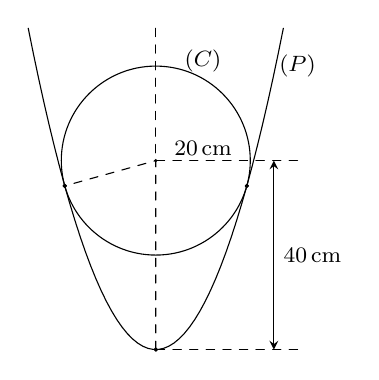
\begin{tikzpicture}[scale=0.6,font=\footnotesize,line join=round,line cap=round,>=stealth]
			\draw (0,4) circle (2 cm);		
			\fill (0,4) circle(1pt);
			\node at (1,6.1) {$(C)$};
			\draw plot[domain=-2.7:2.7,samples=50] (\x, {0.933*\x*\x });
			\node at (3,6) {$(P)$};
			\draw[fill=black](-1.927,3.464) circle(1pt);
			\draw[fill=black](1.927,3.464) circle(1pt);
			\draw[fill=black] (0,0) circle(1pt);
			\draw[dashed] (0,0) -- (0,4) -- (-1.927,3.464);
			\draw[dashed] (0,6.8) -- (0,4) -- (3,4) ;
			\draw[<->, >=stealth] (2.5,4) -- (2.5,0);
			\draw[dashed] (3,0) -- (0,0);
			\node[above] at (1,3.9) {$20$\,cm};
			\node[right] at (2.5,2) {$40$\,cm};		
		\end{tikzpicture}
	}
	\par
	\shortans[0]{39}
	\loigiai{
		\noindent
		\immini{Ta đặt hệ trục $Oxy$ vào với gốc tọa độ $O$ đặt tại đỉnh của parabol, trục tung $Oy$ hướng lên, đi qua tâm đường tròn $(C)$. Như vậy ta sẽ có được tâm đường tròn $(C)$ là $I(0,40)$, bán kính đường tròn $R=20$ cm, phương trình đường tròn $(C)\colon x^2+(y-40)^2=20^2$, với parabol $(P)\colon y=ax^2$ hay $x^2=\dfrac{y}{a}$. Hình được vẽ lại như sau.\\
			Có được hai phương trình trên, ta suy được phương trình tung độ giao điểm là
			\[\dfrac{y}{a} + y^2-80y+40^2-20^2=0.\]
			Vì đường parabol tiếp xúc với đường tròn tại hai điểm có cùng tung độ, đồng nghĩa với việc phương trình bậc hai ở trên có nghiệm kép, tức biệt thức $\Delta = 0$. }{
			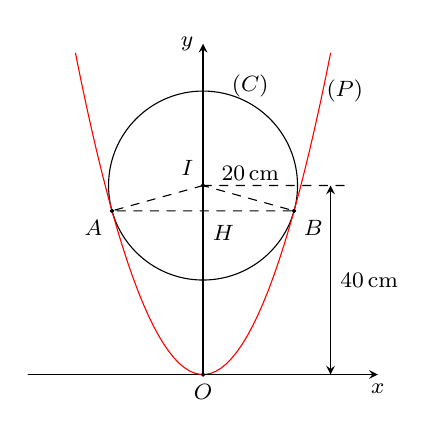
\begin{tikzpicture}[scale=0.6,font=\footnotesize,line join=round,line cap=round,>=stealth]
				\draw[->,>=stealth] (-3.7,0) -- (3.7,0) node[below] {$x$};
				\draw[->,>=stealth] (0,0) -- (0,7) node[left] {$y$};
				\coordinate (O) at (0,0);
				\coordinate (I) at (0,4);
				\coordinate (C) at (0,0);
				\coordinate (A) at (-1.927,3.464);
				\coordinate (B) at (1.927,3.464);
				\coordinate (H) at (0,3);
				\draw (0,4) circle (2 cm);		
				\draw[fill=black](0,4) circle(1pt);
				\node[below] at (O) {$O$};
				\node[above left] at (I) {$I$};
				\node[below left] at (A) {$A$};
				\node[below right] at (B) {$B$};
				\node at (1,6.1) {$(C)$};
				\node[right] at (H) {$H$};
				\node at (3,6) {$(P)$};
				\draw[red] plot[domain=-2.7:2.7,samples=50] (\x, {0.933*\x*\x });
				\draw[fill=black] (A) circle(1pt);
				\draw[fill=black] (B) circle(1pt);
				\draw[fill=black] (O) circle(1pt);
				\draw[dashed] (I) -- (A) -- (B) -- cycle;
				\draw[dashed] (I) -- (3,4) ;
				\draw[<->, >=stealth] (2.7,4) -- (2.7,0);
				\draw[dashed] (3,0) -- (O);
				\node[above] at (1,3.9) {$20$\,cm};
				\node[right] at (2.7,2) {$40$\,cm};		
			\end{tikzpicture}
		}\noindent
		Sau khi thu gọn thành $y^2 - \left( 80-\dfrac{1}{a}\right)y+1200=0$, ta được
		\[\Delta = \left( 80-\dfrac{1}{a}\right)^2-4\cdot 1200 =0 \Rightarrow 80-\dfrac{1}{a} = \sqrt{4\cdot 1200}.\]
		Ta cũng đồng thời có được $y_0= \dfrac{80-\dfrac{1}{a}}{2}=\dfrac{\sqrt{4\cdot 1200}}{2} = 20\sqrt{3}$.\\
		Gọi $H$ là giao điểm giữa $IO$ và $AB$. Ta biết rằng $HO = y_0 = 20\sqrt{3}$, mà tam giác $IAH$ là tam giác vuông, $IA = R = 20$ cm nên ta dễ dàng tính được $AB = 2AH = 2\sqrt{20^2-\left( 40-20\sqrt{3}\right)^2} \approx 39$.
	}
\end{ex}
%%%=============================%%%

%%%=============EX_21=============%%%
\begin{ex}%[1D2C3-6]%[TDMT01]%[Nguyễn Văn Sang]
	Cho hình lập phương $ABCD.A'B'C'D'$ có độ dài cạnh $AB=6$. Gọi $A_1$, $B_1$ lần lượt là hình chiếu của $A$, $B$ trên đường thẳng $CD'$. Gọi $A_2$, $B_2$ lần lượt là hình chiếu của $A_1$, $B_1$ trên đường thẳng $AB$. Gọi $A_3$, $B_3$ lần lượt là hình chiếu của ${A}_2$, $B_2$ trên đường thẳng $A_1B_1 \ldots$ Gọi $A_{n+1}$, $B_{n+1}$ lần lượt là hình chiếu của $A_n$, $B_n$ trên đường thẳng $A_{n-1}B_{n-1}$, ($n \geq 3$). Hãy tính tổng $A_1B_1+A_2B_2+A_3B_3+\ldots$ (\textit{làm tròn kết quả đến hàng phần mười}).
	\par
	\shortans[0]{14,5}
	\loigiai{
		\begin{center}
			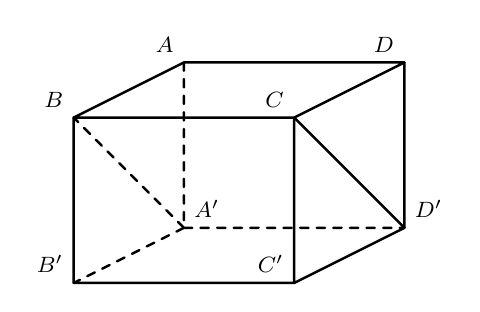
\begin{tikzpicture}[line join=round,line cap=round,line width=0.9pt,font=\footnotesize,scale=0.7]
				\coordinate[label=above left:$A$] (A) at (6,7);
				\coordinate[label=above left:$B$] (B) at (4,6);
				\coordinate[label=above left:$C$] (C) at (8,6);
				\coordinate[label=above left:$D$] (D) at (10,7);
				\coordinate[label=above right:$A'$] (A') at (6,4);
				\coordinate[label=above left:$B'$] (B') at (4,3);
				\coordinate[label=above left:$C'$] (C') at (8,3);
				\coordinate[label=above right:$D'$] (D') at (10,4);
				\draw[smooth] (A)--(B)--(C)--(D)--(A) (C)--(D');
				\draw[dashed] (A')--(B') (A')--(D') (A)--(A') (A')--(B);
				\draw[smooth] (B')--(C')--(D') (B)--(B') (C)--(C')  (D)--(D');		
			\end{tikzpicture}
			\hspace{1cm}
			\begin{tikzpicture}[line join=round,line cap=round,line width=0.9pt,font=\footnotesize,scale=.8]
				% Define coordinates
				\coordinate (O) at (0,0);
				\draw (O) -- (7,0) node[right]{$\Delta_1 \parallel AB$};
				\draw (O) -- (5,5) node[right]{$\Delta_2 \parallel CD'$};
				
				% Points A, B on line Delta_1
				\coordinate[label=below:$A$] (A) at (2,0);
				\coordinate[label=below:$B$] (B) at (5,0);
				\fill (A) circle(1pt);
				\fill (B) circle(1pt);
				
				% Projections A1, B1 on Delta_2
				% Projection of (x,0) onto line y=x is ((x)/2, (x)/2) * sqrt(2)? No.
				% Line is y = x (angle 45). Proj of (x,0) is point P such that OP * vector(1,1) = x * 1? No.
				% Unit vector u = (cos45, sin45). P = (OA . u) u.
				% A(2,0). P = (2 * cos45) * (cos45, sin45) = (2 * 1/sqrt(2)) * (1/sqrt(2), 1/sqrt(2)) = (1,1).
				\coordinate[label=above left:$A_1$] (A1) at (1,1);
				% B(5,0). P = (5 * 1/sqrt(2)) * (1/sqrt(2), 1/sqrt(2)) = (2.5, 2.5).
				\coordinate[label=above left:$B_1$] (B1) at (2.5,2.5);
				\fill (A1) circle(1pt);
				\fill (B1) circle(1pt);
				
				% Projections A2, B2 on Delta_1
				% Proj of (x, y) on x-axis is (x, 0).
				\coordinate[label=below:$A_2$] (A2) at (1,0); 
				\coordinate[label=below:$B_2$] (B2) at (2.5,0);
				\fill (A2) circle(1pt);
				\fill (B2) circle(1pt);
				
				% Draw projection lines
				\draw[dashed] (A)--(A1) (B)--(B1);
				\draw[dashed] (A1)--(A2) (B1)--(B2);
				
				% Mark angles
				\draw (0.5,0) arc (0:45:0.5);
				\node at (0.8,0.3) {$45^\circ$};
				
				% Right angle marks
				\def\size{0.2}
				% At A1 (slope 1). Perpendicular slope -1.
				% Simple mark using coordinate geometry manually or pic
				\draw (A1) -- ++(-45:\size) -- ++(-135:\size) -- ++(135:\size); 
				\draw (B1) -- ++(-45:\size) -- ++(-135:\size) -- ++(135:\size);
				
				% At A2, B2 (straight)
				\draw ($(A2)+(0,\size)$) -- ++(\size,0) -- ++(0,-\size);
				\draw ($(B2)+(0,\size)$) -- ++(\size,0) -- ++(0,-\size);
				
				% Labels for lines
				\node at (3.5, -1) {\textit{(Mô hình minh họa quá trình chiếu)}};
			\end{tikzpicture}
		\end{center}
		\noindent
		Ta có $AB \parallel CD$ (cạnh hình lập phương) nên góc giữa hai đường thẳng $AB$ và $CD'$ bằng góc giữa $CD$ và $CD'$.\\
		Xét hình vuông $CDD'C'$, ta có $CD'$ là đường chéo nên tạo với cạnh $CD$ một góc $45^\circ$. \\
		Suy ra $\varphi = (AB,CD')=(CD,CD')= \widehat{DCD'} = 45^\circ$.\\
		Để dễ hình dung việc tính độ dài các hình chiếu, ta xem hình vẽ minh họa thứ 2 ở trên với $\Delta_1$ đại diện cho phương của $AB$ và $\Delta_2$ đại diện cho phương của $CD'$. Quá trình chiếu \lq\lq ziczac\rq\rq\ diễn ra như sau
		\begin{itemize}
			\item $A_1$, $B_1$ là hình chiếu của $A$, $B$ trên $CD'$ $\Rightarrow$ Độ dài bị thu hẹp bởi hệ số $\cos 45^\circ$. \\
			Ta có $A_1B_1 = AB \cdot \cos 45^\circ$.
			\item $A_2$, $B_2$ lại là hình chiếu của $A_1, B_1$ ngược trở lại phương $AB$ $\Rightarrow$ Độ dài tiếp tục bị nhân thêm $\cos 45^\circ$.\\
			Ta có $A_2B_2 = A_1B_1 \cdot \cos 45^\circ = AB \cdot (\cos 45^\circ)^2$.
			\item Tương tự, $A_3B_3 = AB \cdot (\cos 45^\circ)^3$, $\ldots$, $A_nB_n = AB \cdot (\cos 45^\circ)^n$.
		\end{itemize}
		Dãy số $u_n = A_n B_n$ lập thành một cấp số nhân lùi vô hạn với
		\begin{itemize}
			\item Số hạng đầu $u_1 = A_1B_1 = 6 \cdot \dfrac{\sqrt{2}}{2} = 3\sqrt{2}$.
			\item Công bội $q = \cos 45^\circ = \dfrac{\sqrt{2}}{2} < 1$.
		\end{itemize}
		Tổng các độ dài hình chiếu là
		\[S = A_1B_1 + A_2B_2 + A_3B_3 + \dots = \dfrac{u_1}{1-q} = \dfrac{3\sqrt{2}}{1-\dfrac{\sqrt{2}}{2}}\approx 14{,}5.\]
	}
\end{ex}
%%%=============================%%%

%%%=============EX_22=============%%%
\begin{ex}%[2D6V1-3]%[TDMT01]%[Mui Doan]
	Cho hai hộp đựng các viên bi cùng kích thước, cùng khối lượng, cùng màu. Hộp I đựng $6$ viên bi có đánh số $1$, $2$, $3$, $4$, $5$, $7$ và hộp II có đựng $6$ viên bi được đánh số $1$, $2$, $3$, $4$, $5$, $6$. Bạn An lấy ngẫu nhiên $4$ viên bi từ hộp I, bạn Bình lấy ngẫu nhiên $4$ viên bi từ hộp II. Sau đó các bạn sẽ sắp xếp các chữ số ghi trên các viên bi mà mình lấy được thành một số tự nhiên có $4$ chữ số giảm dần. Tính xác suất để số tự nhiên của Bình lớn hơn số tự nhiên của An (\textit{làm tròn kết quả đến hàng phần trăm}).
	\begin{center}
		\vspace{-6pt}
		\noindent
		\begin{tikzpicture}[scale=0.95,
			bi/.style={
				circle,
				draw=black,
				thick,
				minimum size=6mm,
				ball color=gray!40,
				font=\small\bfseries,
				text=white
			}
			]			
			%---------------- HỘP I ----------------
			\node at (5,4.6) {\bf HỘP I};
			\draw[thick] (3,4)--(7,4)--(7,2)--(3,2)--cycle;			
			\node[bi] at (6.2,2.46) {1};
			\node[bi] at (6.14,3.5) {2};
			\node[bi] at (4.96,2.36) {3};
			\node[bi] at (3.6,2.46) {4};
			\node[bi] at (4.5,3.26) {7};
			\node[bi] at (3.56,3.46) {5};			
			%---------------- HỘP II ----------------
			\node at (11,4.6) {\bf HỘP II};
			\draw[thick] (9,4)--(13,4)--(13,2)--(9,2)--cycle;			
			\node[bi] at (12.04,2.54) {1};
			\node[bi] at (10.48,2.62) {3};
			\node[bi] at (9.44,2.46) {4};
			\node[bi] at (9.7,3.46) {5};
			\node[bi] at (10.88,3.51) {6};
			\node[bi] at (12.17,3.6) {2};			
		\end{tikzpicture}
		\vspace{-8pt}
	\end{center}
	\par
	\shortans[0]{0,27}
	\loigiai{ 
		Gọi $A$ là \lq\lq biến cố số tự nhiên An lớn hơn Bình\rq\rq.\\
		Gọi $B$ là \lq\lq biến cố số tự nhiên An bé hơn Bình\rq\rq.\\
		Gọi $C$ là \lq\lq biến cố số tự nhiên bằng nhau\rq\rq.\\
		Ta có số phần tử của không gian mẫu là $n(\Omega)=\mathrm{C}_6^4 \mathrm{C}_6^4 =225$.\\
		\begin{itemize}
			\item \textbf{Cách 1:} Các số có thể tạo thành từ hộp I thoả điều kiện giảm dần là
			\[
			\begin{aligned}
				A_1=\{&4321,\,5321,\,7321,\,5421,\,7421,\,7521,\,5431,\,7431,\,7531,\,7541,\\
				&5432,\,7432,\,7532,\,7542,\,7543\}.
			\end{aligned}
			\]
			Các số có thể tạo thành từ hộp II thoả điều kiện giảm dần là
			\[
			\begin{aligned}
				B_1=\{&4321,\,5321,\,6321,\,5421,\,6421,\,6521,\,5431,\,6431,\,6531,\,6541,\\
				&5432,\,6432,\,6532,\,6542,\,6543\}.
			\end{aligned}
			\]
			Sắp xếp theo thứ tự tăng dần
			\[
			\begin{aligned}
				A_1=\{&4321,\,5321,\,5421,\,5431,\,5432,\,7321,\,7421,\,7431,\,7432,\\
				&7521,\,7531,\,7532,\,7541,\,7542,\,7543\}.\\[4pt]
				B_1=\{&4321,\,5321,\,5421,\,5431,\,5432,\,6321,\,6421,\,6431,\,6432,\\
				&6521,\,6531,\,6532,\,6541,\,6542,\,6543\}.
			\end{aligned}
			\]
			Ta đếm số trường hợp để số của Bình lớn hơn số của An (tức là biến cố $B$):
			\[
			\begin{array}{c|c}
				\text{Số của An} & \text{Số cách để Bình lớn hơn An} \\ \hline
				4321 & 14\\
				5321 & 13\\
				5421 & 12\\
				5431 & 11\\
				5432 & 10\\
				7321 & 5\\
				7421 & 4\\
				7431 & 3\\
				7432 & 2\\
				7521 & 2\\
				7531 & 1\\
				7532 & 0\\
				7541 & 0\\
				7542 & 0\\
				7543 & 0
			\end{array}
			\]
			Do đó $	n(B)=14+13+12+11+10+5+4+3+2+2+1=60$.\\
			Suy ra $\mathrm{P}(B)=\dfrac{n(B)}{n(\Omega)}=\dfrac{60}{225}\approx 0{,}27$.
			\item \textbf{Cách 2:} Vì $A$, $B$, $C$ là ba biến cố xung khắc và đầy đủ nên
			\[
			\mathrm{P}(A)+\mathrm{P}(B)+\mathrm{P}(C)=1
			\]
			Ta có sơ đồ cây\\
			\begin{tikzpicture}[
				grow=right, 
				level distance=4cm, 
				level 1/.style={sibling distance=4cm}, 
				level 2/.style={sibling distance=2.5cm, level distance=7cm}
				]
				\node {Gốc}
				child {
					node {An lấy được $7$}
					child { node {A: $\mathrm{C}_5^3 \mathrm{C}_6^4$} 
						edge from parent node[auto, swap] {$A>B$}}
				}
				child {
					node {$\heva{ & A \, \textbf{ An lấy được} \, 1,2,3,4,5 \\
							& B \textbf{ Bình lấy được 6} \ }$}
					child { node {B: $\mathrm{C}_5^3 \mathrm{C}_5^4=50$} 
						edge from parent node[auto, swap] {$A<B$}}
				}
				child {
					node {An, Bình lấy được $4$ số từ $1$, $2$, $3$, $4$, $5$ }
					child { node { C $ \left( A=B \right): \, \mathrm{C}_5 ^4 =5 $ } }
					child { node {B $ \left( A<B \right) \, \textbf{có 10 cách} $ } }
					child { node {A $ \left( A>B \right)\, \textbf{có 10 cách} $}  }
				};
			\end{tikzpicture}\\
			Xác suất cần tính $\mathrm{P}(B)=\dfrac{n(B)}{n(\Omega)}= \dfrac{50+10}{225}=\dfrac{4}{15}\approx 0{,}27$.
		\end{itemize}
	}
\end{ex}
%%%=============================%%%
\Closesolutionfile{ans}
\newpage

\indapan{12}{ans/ansTN-Dung}
\indapan[TF]{2}{ans/ansTN-DungSai}
\indapan[SA]{6}{ans/ansTN-DienKhuyet}
%%%%%%%%%%%%%%
%%nhãn kết thúc đề (để đếm số trang tự động mỗi đề)
\label{B\thedeso}